%=========================================================================
% PREAMBLE
% =========================================================================
\documentclass[12pt, a4paper]{article}

\usepackage{amsmath, amssymb}
\usepackage{geometry}
\usepackage{tikz}
\usepackage{circuitikz}
\usepackage{booktabs}
\usepackage{array}
\usepackage{enumitem}
\usepackage{xcolor}
\usepackage{tcolorbox}
\usepackage{hyperref}
\usepackage{fancyhdr}
\usepackage{tabularx}
\usepackage{makecell}
\geometry{margin=2.5cm}
\setlength{\headheight}{14.5pt}
\usetikzlibrary{circuits.logic.US, positioning, arrows.meta, shapes.gates.logic.US}

% ---- Custom colours ----
\definecolor{gateblue}{RGB}{0, 70, 127}
\definecolor{answergreen}{RGB}{0, 120, 60}
\definecolor{shadegray}{RGB}{245, 245, 245}

% ---- Fancy header ----
\pagestyle{fancy}
\fancyhf{}
\lhead{\textbf{Digital Logic -- GATE EC}}
\rhead{Majority Logic Gate (Q.23)}
\cfoot{\thepage}



% =========================================================================
% CUSTOM MACROS (mirrors the style used in the reference document)
% =========================================================================
\newcommand{\qstart}[2]{%
  \begin{tcolorbox}[colback=shadegray, colframe=gateblue,
      title={\textbf{#1}}, fonttitle=\bfseries\large, arc=4pt,
      left=6pt, right=6pt, top=4pt, bottom=4pt]
  #2
}
\newcommand{\qcont}[1]{#1}
\newcommand{\qopt}[2]{\par\medskip\textbf{#1}\quad #2}
\newcommand{\qend}{\end{tcolorbox}}

\usetikzlibrary{circuits.logic.US, positioning, arrows.meta, shapes.gates.logic.US}


% =========================================================================
% DOCUMENT BEGINS
% =========================================================================
\begin{document}

% =========================================================================
% QUESTION BLOCK
% =========================================================================
\qstart{Q.23}{%
  A 3-input \textbf{majority logic gate} has inputs $X$, $Y$, and $Z$.
  The output $F$ of the gate is logic `\textbf{1}' if \emph{two or more}
  of the inputs are logic `1'. The output $F$ is logic `\textbf{0}' if
  two or more of the inputs are logic `0'.

  \medskip
  Which one of the following options is a Boolean expression of the
  output $F$?%
}

\qcont{%
  \begin{center}
    \renewcommand{\arraystretch}{1.5}
    \begin{tabular}{|c|p{8cm}|}
      \hline
      (A) & $XY + YZ + ZX$ \\
      \hline
      (B) & $X \oplus Y \oplus Z$ \\
      \hline
      (C) & $X + Y + Z$ \\
      \hline
      (D) & $XYZ$ \\
      \hline
    \end{tabular}
  \end{center}
}
\qend

% =========================================================================
% TRUTH TABLE
% =========================================================================
\section*{Truth Table for the 3-Input Majority Function}

The majority function activates its output whenever at least two of the
three inputs are logic~1. The complete truth table is given below.

\begin{center}
  \renewcommand{\arraystretch}{1.3}
  \begin{tabular}{|c|c|c||c|c|}
    \hline
    \textbf{X} & \textbf{Y} & \textbf{Z} &
    \textbf{Majority count} & \textbf{F} \\
    \hline
    0 & 0 & 0 & 0 ones & 0 \\
    0 & 0 & 1 & 1 one & 0 \\
    0 & 1 & 0 & 1 one & 0 \\
    0 & 1 & 1 & 2 ones & \textbf{1} \\
    1 & 0 & 0 & 1 one & 0 \\
    1 & 0 & 1 & 2 ones & \textbf{1} \\
    1 & 1 & 0 & 2 ones & \textbf{1} \\
    1 & 1 & 1 & 3 ones & \textbf{1} \\
    \hline
  \end{tabular}
\end{center}

\medskip
The four minterms where $F=1$ are: $m_3,\,m_5,\,m_6,\,m_7$.
% =========================================================================
% LOGIC CIRCUIT DIAGRAM
% =========================================================================
\section*{Logic Circuit Diagram of the Majority Gate}

\begin{center}
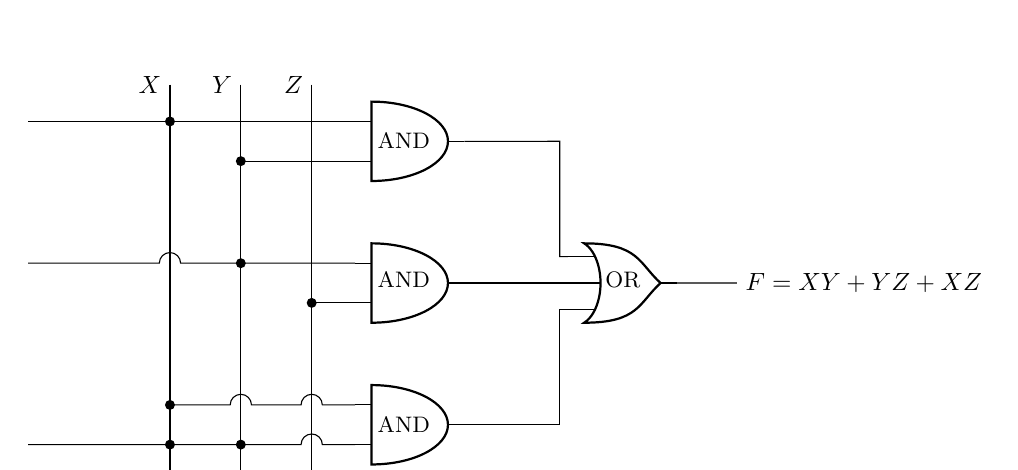
\begin{tikzpicture}[scale=0.9, transform shape]

% Define logic gates
\node[and port] (and1) at (5, 4) {};
\node[and port] (and2) at (5, 2) {};
\node[and port] (and3) at (5, 0) {};
\node[or port, number inputs=3] (or1) at (8, 2) {};

% Vertical bus lines
\draw (1, 4.8) -- (1, -0.8);
\draw (2, 4.8) -- (2, -0.8);
\draw (3, 4.8) -- (3, -0.8);

% Input labels
\node[left] at (1,4.8) {$X$};
\node[left] at (2,4.8) {$Y$};
\node[left] at (3,4.8) {$Z$};

% Gate labels
\node at (4.3,4) {\small AND};
\node at (4.3,2.04) {\small AND};
\node at (4.3,0) {\small AND};

\node at (7.39,2.04) {\small OR};

% Connections to Top AND Gate (XY)
\draw let \p1=(and1.in 1) in (-1,\y1) -- (\p1);
\path let \p1=(and1.in 1) in coordinate (t1) at (1,\y1);
\fill (t1) circle (2pt);

\draw let \p1=(and1.in 2) in (2,\y1) -- (\p1);
\path let \p1=(and1.in 2) in coordinate (t2) at (2,\y1);
\fill (t2) circle (2pt);

% Connections to Middle AND Gate (YZ)
\draw let \p1=(and2.in 1) in (-1,\y1) -- (0.85,\y1)
      arc (180:0:0.15) -- (\p1);
\path let \p1=(and2.in 1) in coordinate (m1) at (2,\y1);
\fill (m1) circle (2pt);

\draw let \p1=(and2.in 2) in (3,\y1) -- (\p1);
\path let \p1=(and2.in 2) in coordinate (m2) at (3,\y1);
\fill (m2) circle (2pt);

% Connections to Bottom AND Gate (XZ)
\draw let \p1=(and3.in 1) in (1,\y1) -- (1.85,\y1)
      arc (180:0:0.15) -- (2.85,\y1)
      arc (180:0:0.15) -- (\p1);
\path let \p1=(and3.in 1) in coordinate (b1) at (1,\y1);
\fill (b1) circle (2pt);

\draw let \p1=(and3.in 2) in (-1,\y1) -- (2.85,\y1)
      arc (180:0:0.15) -- (\p1);
\path let \p1=(and3.in 2) in coordinate (b2a) at (1,\y1);
\path let \p1=(and3.in 2) in coordinate (b2b) at (2,\y1);
\fill (b2a) circle (2pt);
\fill (b2b) circle (2pt);

% Outputs of AND gates to OR gate
\draw (and1.out) -- (6.5,4) |- (or1.in 1);
\draw (and2.out) -- (or1.in 2);
\draw (and3.out) -- (6.5,0) |- (or1.in 3);

% Final output
\draw (or1.out) -- (9.0,2);
\node[right] at (9.0,2) {$F = XY + YZ + XZ$};

\end{tikzpicture}
\end{center}


% =========================================================================
% DETAILED MATHEMATICAL DERIVATION
% =========================================================================
\section*{Step-by-Step Mathematical Solution}

\begin{enumerate}[label=\textbf{Step \arabic*.}, leftmargin=*, itemsep=8pt]

  % ------------------------------------------------------------------
  \item \textbf{Build the Sum of Minterms (Canonical SOP)}

  From the truth table the function is HIGH for minterms 3, 5, 6, 7:
  \begin{equation}
    F = \sum m(3,\,5,\,6,\,7)
      = \overline{X}YZ + X\overline{Y}Z + XY\overline{Z} + XYZ
  \end{equation}

  % ------------------------------------------------------------------
  \item \textbf{Apply Boolean Algebra — Group Pairs}

  Group $XYZ$ with each of the three other minterms:
  \begin{align}
    \text{Group 1:}\quad XY\overline{Z} + XYZ &= XY(\overline{Z}+Z) = XY \\
    \text{Group 2:}\quad X\overline{Y}Z + XYZ &= XZ(\overline{Y}+Y) = XZ \\
    \text{Group 3:}\quad \overline{X}YZ + XYZ &= YZ(\overline{X}+X) = YZ
  \end{align}

  % ------------------------------------------------------------------
  \item \textbf{Combine the Grouped Terms}

  Using the absorption law $A + A = A$ (the term $XYZ$ is used three times but each
  pair is valid by the idempotency of Boolean OR):
  \begin{equation}
    \boxed{F = XY + YZ + ZX}
  \end{equation}

  % ------------------------------------------------------------------
  \item \textbf{Verify Against All Minterms}

  \begin{center}
    \renewcommand{\arraystretch}{1.3}
    \begin{tabular}{|c|c|c||c|c|c||c|}
      \hline
      $X$ & $Y$ & $Z$ & $XY$ & $YZ$ & $ZX$ & $F = XY+YZ+ZX$ \\
      \hline
      0 & 0 & 0 & 0 & 0 & 0 & \textbf{0} \\
      0 & 0 & 1 & 0 & 0 & 0 & \textbf{0} \\
      0 & 1 & 0 & 0 & 0 & 0 & \textbf{0} \\
      0 & 1 & 1 & 0 & 1 & 0 & \textbf{1} \\
      1 & 0 & 0 & 0 & 0 & 0 & \textbf{0} \\
      1 & 0 & 1 & 0 & 0 & 1 & \textbf{1} \\
      1 & 1 & 0 & 1 & 0 & 0 & \textbf{1} \\
      1 & 1 & 1 & 1 & 1 & 1 & \textbf{1} \\
      \hline
    \end{tabular}
  \end{center}
  The verification confirms that $F = XY + YZ + ZX$ matches the truth
  table exactly.

  % ------------------------------------------------------------------
  \item \textbf{Eliminate the Incorrect Options}

  \begin{itemize}
    \item \textbf{(B) $X \oplus Y \oplus Z$:} XOR of three inputs gives
          the \emph{odd-parity} function, which outputs~1 for minterms 1, 2, 4, 7
          — not the same as the majority function.
    \item \textbf{(C) $X + Y + Z$:} OR of inputs is HIGH as long as
          \emph{any} input is~1, including the case $(0,0,1)$ where the
          majority is 0. This over-counts.
    \item \textbf{(D) $XYZ$:} AND of all inputs is HIGH only when
          \emph{all three} inputs are~1. This under-counts.
  \end{itemize}
\end{enumerate}

\begin{tcolorbox}[colback=answergreen!8, colframe=answergreen,
    title={\textbf{Correct Answer}}, fonttitle=\bfseries]
  \textbf{Option (A):} $F = XY + YZ + ZX$

  This is the standard 3-input \textbf{majority function}, implemented with
  three 2-input AND gates whose outputs feed a 3-input OR gate.
\end{tcolorbox}

% =========================================================================
% HARDWARE INTEGRATION GUIDE
% =========================================================================
\newpage
\section*{Hardware Implementation Blueprint}

\subsection*{1. Bill of Materials}
\begin{itemize}
  \item 1$\times$ Arduino UNO Development Board
  \item 1$\times$ Solderless Breadboard
  \item 3$\times$ Tactile Push Buttons (Inputs $X$, $Y$, and $Z$)
  \item 3$\times$ $10\,\text{k}\Omega$ Pull-down Resistors
  \item 1$\times$ Light-Emitting Diode (LED — Output $F$)
  \item 1$\times$ $220\,\Omega$ Current-Limiting Resistor
  \item Solid-core hookup jumper wires
  \item \textit{Optional:} 74HC08 (Quad 2-input AND) + 74HC32 (Quad 2-input OR) ICs
\end{itemize}

\subsection*{2. Step-by-Step Pin Mapping \& Wiring}

\begin{itemize}
  \item \textbf{Input Sub-circuit (Push Buttons):}
  \begin{itemize}
    \item Bridge Push Button $X$ across the breadboard centre channel.
          Connect one high-side terminal to the Arduino \textbf{5V} rail.
          Connect the opposite low-side terminal to Arduino
          \textbf{Digital Pin 2}. Tie a $10\,\text{k}\Omega$ pull-down
          resistor from Pin 2 to the common \textbf{GND} rail.
    \item Position Push Button $Y$ identically, wired to
          \textbf{Digital Pin 3}, with its own $10\,\text{k}\Omega$
          pull-down resistor to \textbf{GND}.
    \item Position Push Button $Z$ identically, wired to
          \textbf{Digital Pin 4}, with its own $10\,\text{k}\Omega$
          pull-down resistor to \textbf{GND}.
  \end{itemize}
  \item \textbf{Output Sub-circuit (LED Indicator):}
  \begin{itemize}
    \item Route a jumper wire from Arduino \textbf{Digital Pin 5} to an
          empty row on the breadboard. Connect the $220\,\Omega$
          current-limiting resistor from this row to the positive anode
          leg (longer lead) of the LED.
    \item Connect the shorter cathode leg of the LED straight to the
          common \textbf{GND} rail. Complete the loop by linking the
          breadboard \textbf{GND} rail to an Arduino \textbf{GND} pin.
  \end{itemize}
\end{itemize}

\subsection*{3. Hardware Block Diagram}

\begin{center}
\begin{circuitikz}[american, scale=0.85, transform shape, font=\sffamily]

    % --- Power Rails (Parallel Lines) ---
    % Top 5V Rail
    \draw[thick] (-7.5, 6) -- (10, 6);
    \draw[thick] (-7.5, 6.1) -- (10, 6.1);
    \node[left, font=\bfseries] at (-7.5, 6.05) {5V};
    \node[right, font=\bfseries] at (10, 6.05) {5V};

    % Bottom GND Rail
    \draw[thick] (-7.5, -2) -- (10, -2);
    \draw[thick] (-7.5, -2.1) -- (10, -2.1);
    \node[right, font=\bfseries] at (10, -2.05) {GND};
    
    % Grounding symbol on left bottom
    \draw[thick] (-7.5, -2) -- (-8, -2);
    \node[ground] at (-8, -2) {};

    % --- Arduino Uno Block ---
    \draw[thick, fill=white] (0, 0) rectangle (4, 4);
 \node[align=center] at (2, 2.0) {\Large Arduino\\Uno};
    
    % Arduino Pins
    \node[below] at (2, 4) {5V};
    \node[above] at (2, 0) {GND};
    \node[right] at (0, 3.2) {D2};
    \node[right] at (0, 2.4) {D3};
    \node[right] at (0, 1.6) {D4};
    \node[left] at (4, 2.4) {D5};

    % Arduino Power Connections
    \draw[thick] (2, 4) -- (2, 6);
    \draw[fill=black] (2, 6) circle (2pt);
    \draw[thick] (2, 0) -- (2, -2);
    \draw[fill=black] (2, -2) circle (2pt);

    % --- Input Circuit (Left) ---
    % Vertical 5V supply drop
    \draw[thick] (-5.5, 6) -- (-5.5, 1.6);
    \draw[fill=black] (-5.5, 6) circle (2pt);

    


% SW1 (X)
\draw[thick] (-5.5, 3.2) -- (-5.0, 3.2);
\draw[fill=black] (-5.5, 3.2) circle (2pt);
\draw[thick] (-5.0, 3.2) to[spst] (-3.5, 3.2);

% SW2 (Y)
\draw[thick] (-5.5, 2.4) -- (-5.0, 2.4);
\draw[fill=black] (-5.5, 2.4) circle (2pt);
\draw[thick] (-5.0, 2.4) to[spst] (-3.5, 2.4);

% SW3 (Z)
\draw[thick] (-5.5, 1.6) -- (-5.0, 1.6);
\draw[fill=black] (-5.5, 1.6) circle (2pt);
\draw[thick] (-5.0, 1.6) to[spst] (-3.5, 1.6);




    % Signal Lines & Pull-down Resistors
    % D2
    \draw[thick] (-4.2, 3.2) -- (0, 3.2);
    \draw[fill=black] (-4.2, 3.2) circle (2pt);
    \draw[thick] (-4.2, 3.2) to[R, l=R1, a=10k$\Omega$] (-4.2, -2);
    \draw[fill=black] (-4.2, -2) circle (2pt);

    % D3
    \draw[thick] (-3.5, 2.4) -- (0, 2.4);
    \draw[fill=black] (-2.3, 2.4) circle (2pt);
    \draw[thick] (-2.3, 2.4) to[R, l=R2, a=10k$\Omega$] (-2.3, -2);
    \draw[fill=black] (-2.3, -2) circle (2pt);

    % D4
    \draw[thick] (-3.5, 1.6) -- (0, 1.6);
    \draw[fill=black] (-0.77, 1.6) circle (2pt);
    \draw[thick] (-0.77, 1.6) to[R, l=R3, a=10k$\Omega$] (-0.77, -2);
    \draw[fill=black] (-0.77, -2) circle (2pt);

    % --- Output Circuit (Right) ---
    % D5 Signal Path
    \draw[thick] (4, 2.4) -- (4.5, 2.4);
    \draw[thick] (4.5, 2.4) to[R, l=R4, a=220$\Omega$] (6.5, 2.4);
    \draw[thick] (6.5, 2.4) to[led, l=LED1] (8.5, 2.4);
    \draw[thick] (8.5, 2.4) -- (8.5, -2);
    \draw[fill=black] (8.5, -2) circle (2pt);

\end{circuitikz}
\end{center}

\subsection*{4. Arduino Sketch (Software Logic)}

The sketch below reads the three push-button inputs, computes the
majority function $F = XY + YZ + ZX$ in firmware, and drives the LED:

\begin{tcolorbox}[colback=gray!5, colframe=gray!60,
    title={\textbf{Project Source \& Links}}, fonttitle=\bfseries]
\textbf{repo link:} \url{https://github.com/Harshith-Akella-1/gate-q.git} \\[0.5em]
\textbf{assembly file link:} \url{https://github.com/Harshith-Akella-1/gate-q/blob/main/gate-q.asm} \\[0.5em]
\textbf{arduino files link:} \url{https://github.com/Harshith-Akella-1/gate-q/blob/main/gate-q.ino}
\end{tcolorbox}

\subsection*{5. Connection Architecture Summary}

\begin{itemize}
  \item \textbf{Power Distribution Rails:} The Arduino 5V and GND pins
        tie directly into the breadboard power rails to deliver stable
        voltage across all three inputs and the output sub-circuit.
  \item \textbf{Input X Configuration (Pin 2):} Push Button $X$ links to
        Digital Pin 2 with a $10\,\text{k}\Omega$ pull-down to GND,
        ensuring a clean logic~0 when the button is released.
  \item \textbf{Input Y Configuration (Pin 3):} Push Button $Y$ hooks
        into Digital Pin 3 with an identical $10\,\text{k}\Omega$
        pull-down arrangement.
  \item \textbf{Input Z Configuration (Pin 4):} Push Button $Z$ connects
        to Digital Pin 4 with the same pull-down scheme.
  \item \textbf{Output F Signal Path (Pin 5):} The computed majority
        result is driven from Digital Pin 5 through a $220\,\Omega$
        current-limiting resistor to the LED anode, with the cathode
        returning to the common GND rail. The LED illuminates whenever
        $F = 1$, i.e., when two or more of the three inputs are pressed.
\end{itemize}

\end{document}
